\section{Part I: Data Cleaning and Preprocessing (for dataset A)}
\subsection{Detecting Issues in the dataset}
For this part of the assignment, the dataset had to be analyzed first as part of the preprocessing step to detect issues such as missing values and outliers. There was found to be a 124053 missing values and 14622 outliers in the dataset. Columns and rows that had all NaN values were checked and there was found to be three columns (fea.34, fea.35, fea.36) and 795 rows (samples) that were missing 70\% of the features.
Outliers were found by first finding the standard deviation of each feature and then using each standard deviation to find values in that specific feature that vary by more than 3 standard deviations. 

\subsection{Fixing Issues}
Columns: fea.34, fea.35, fea.36 were dropped from the dataset as they were entirely NaN values. Then the rows (samples) that had all NaN values (795 samples) were dropped from the dataset. After dropping those columns and rows, the number of the missing values reduced from 124,053 to 6048 and the data size reduced to 18205*78 (18205 samples and 78 features). 
After that, the outliers had to be checked and taken care of before replacing the 6048 missing values with the mean as the outliers would effect the mean. There were over 14000 data points (makes ~1 percent of the entire data) that vary from the features mean by over 3 standard deviations. Since the nature of the experiment is not well defined, those outliers are assumed to be noise detected by the motion sensors. After the detection of the outliers, they were replaced with the mean of each feature. Final step was to replace all the missing values denoted by NA with the mean of each feature after the outliers were taken care of. 

\subsection{Normalizing Data}
Figure~\ref{fig:fig1} shows the comparison between histogram plots of feature 9 and 24 before and after normalization. The large spike is a result of multiple data points (outliers and missing values) being set to the mean value.
\begin{itemize}
\item min/max has range from 0 to 1
\item z-score is centered around mean = 0 and is ideal for PCA
\item all histograms have the same shape after cleaning
\item feat 24 seems to look normally distributed, feat 9 is not
\end{itemize}


%%%%%%%%%%%%%%%%%%%%%%%%%%%%%%%%%%%%%%%%%%%%%%%%%%%%%%%%%%%%%%%%%%%
%
% Commands to include a figure:
%
%%%%%%%%%%%%%%%%%%%%%%%%%%%%%%%%%%%%%%%%%%%%%%%%%%%%%%%%%%%%%%%%%%%

\begin{figure}[!ht]
 \centering
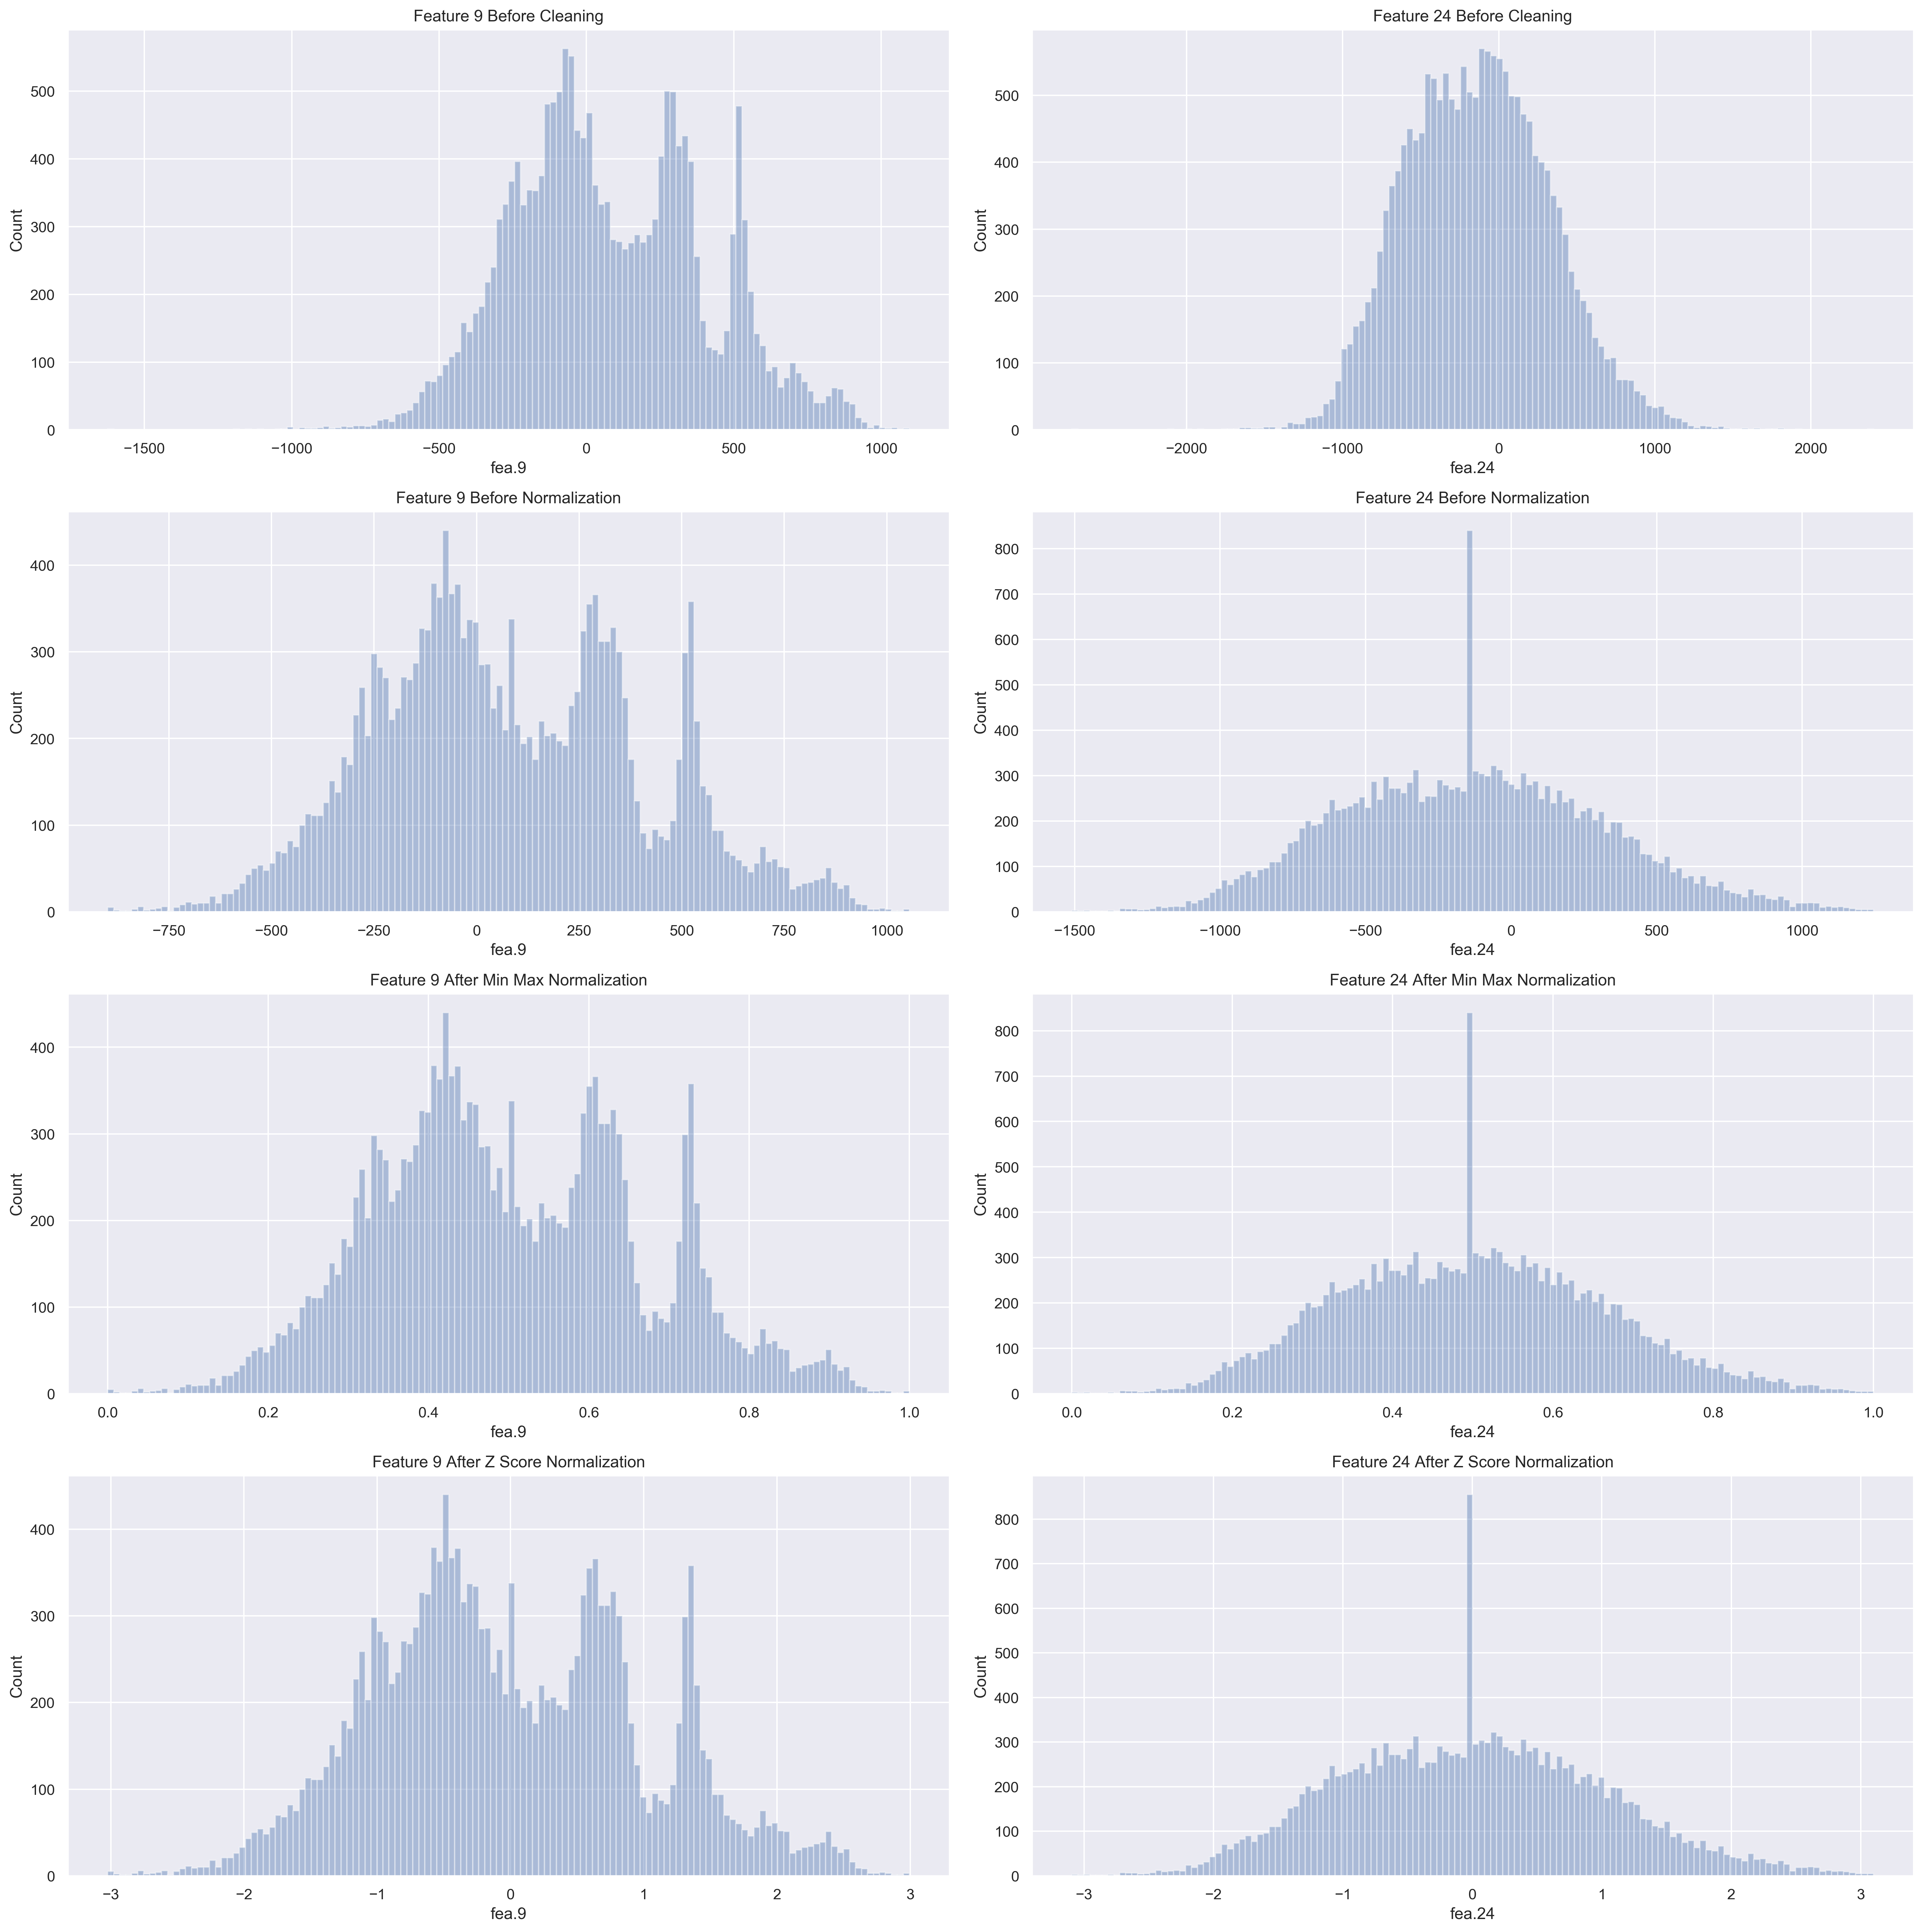
\includegraphics[width=6.1in]{assignment1/1-3-histograms.png}
\caption{\label{fig:fig1}histogram plots of feature 9 and 24 before and after normalization}
\end{figure}
